\documentclass[12pt]{amsart}

\usepackage{ljm-auth}
\usepackage{graphicx}

\usepackage{epsf}
\usepackage{epstopdf}

\newtheorem{definition}{Definition}
\newtheorem{theorem}{Theorem}
\newtheorem{corollary}{Corollary}
\newtheorem{lemma}{Lemma}


\author{ L.\,I.\,Ivanovsky$^{1,2}$ }
\crauthor{ Ivanovsky } % for running heads

\tit{Stable regimes of dynamic systems with impulsive influences}
\shorttit{Stable regimes of impulsive systems } %for running heads

\setcounter{page}{3}

\begin{document}

\maketit

\address{
$^1$  Yaroslavl State University, Sovetskaya str., 14, Yaroslavl, 150000, Russia,
$^2$  Scientific Center in Chernogolovka RAS, Lesnaya str., 9, Chernogolovka, Moscow region, 142432, Russia,
}

\email{leon19unknown@gmail.com}

\Received{27.09.2016}

\abstract{
Let us consider a mathematical model of dynamic system, which is presented as a chain of three connected, singularly perturbed nonlinear differential equations. In the further text there were researched the questions of existence and stability of periodic solutions of this system due to a bifurcational analysis of special two-dimensional map. Also the special attention is paid to the number of coexisting stable regimes.
}

\notes{0}{
\subclass{35B40, 35B41, 65M06} % 2010 Mathematical Subject Classification
\keywords{phase portraits, 
stable regimes, 
bifurcations}%
\thank{This work was supported by the Russian Science Foundation (project no. 14-21-00158)} }

\section{Problem definition}\label{sec:1}
Let us consider a chain of three connected, singularly perturbed oscillators with a delay:
\begin{equation}\label{u_system} 
	\dot{u_j} = d(a_1u_{j-1}-a_2u_j+u_{j+1})+\lambda(-1+\alpha f(u_j(t-1)) - \beta g(u_j))u_j, \quad j = \overline{1,3},
\end{equation}
where $ u_j = u_j(t) > 0 $, parameters $ a_1, a_2 \in \{ 0, 1, 2 \}, \lambda \gg 1, \beta > 0, \alpha > 1 + \beta $ and smooth functions $ f(u), g(u) \in C^2(\mathbb{R}_+) $ have entry conditions: $ 0 < \beta g(u) < \alpha, f(0) = g(0) = 1 $ and  $ f(u), g(u), uf'(u), ug'(u) = O(1/u) $ as $ u \rightarrow +\infty $. In this article there are researched three types of system \eqref{u_system} for different values of parameters $ a_1, a_2 $ and conditions on $ u_0, u_4 $: a) $ a_1 = 1, a_2 = 2, u_0 = u_1, u_3 = u_4 $; b) $ a_1 = 1, a_2 = 2, u_0 = u_3, u_1 = u_4 $; c) $ a_1 = 0, a_2 = 1, u_1 = u_4 $.

In articles [1--3] there was proved, when $ \lambda $ is sufficiently great, by means of following substitutions
$$ u_1 = \mbox{exp}\left(\frac{x}{\varepsilon}\right), \; u_j = \mbox{exp}\left(\frac{x}{\varepsilon} + \sum_{k=1}^{j-1}y_k\right), \; j= 2,3, \quad \varepsilon = \frac{1}{\lambda}\ll 1, $$
where $ x, y_1, ..., y_{m-1} $ are new variables, system \eqref{u_system} can be transformed to the two-dimensional system of differential equations without small parameters, but with impulsive influences 
\begin{equation}\label{y_system}
\begin{array}{l}
\dot{y_1} = d(e^{y_2} + a_1e^{-y_1} - e^{y_1} - a_1e^{-y_0}), \\
\dot{y_2} = d(e^{y_3} + a_1e^{-y_2} - e^{y_2} - a_1e^{-y_1}),
\end{array}
\end{equation}
$$ y_j(+0) = \frac{\alpha -1}{\alpha - \beta - 1}y_j(-0), \quad y_j(1+0) = y_j(1-0) - \frac{\alpha}{\alpha - 1}y_j(+0), $$
$$ y_j(\alpha + 0) = (1 + \beta)y_j(\alpha - 0), \quad y_j(\alpha + 1 + 0) = y_j(\alpha + 1 - 0) - \frac{\alpha}{1 + \beta}y_j(\alpha + 0),  $$
where values of $ y_0, y_3 $ depend on entry conditions on $ u_0 $ and $ u_4 $: a) $ u_0 = u_1, u_3 = u_4 $: $ y_0 = y_3 = 0 $; b) $ u_0 = u_3, u_1 = u_4 $: $ y_0 = y_3 = -(y_1 + y_2) $; c) $ u_1 = u_4 $: $ y_3 = -(y_1 + y_2) $.

Let us consider solutions of system \eqref{y_system} $ y_1(t, z_1, z_2), y_2(t, z_1, z_2) $ with entry conditions $ y_1(-0, z_1, z_2) = z_1, y_2(-0, z_1, z_2) = z_2 $. For map
\begin{equation}\label{phi_map}
	\Phi(z): \begin{pmatrix}
           z_1 \\
           z_2
          \end{pmatrix}
					\to
					\begin{pmatrix}
           y_1(T_0, z_1, z_2) \\
           y_2(T_0, z_1, z_2)
          \end{pmatrix}
\end{equation}
in articles [1--3] there was proved, that exponentially stable points of map \eqref{phi_map} are satisfied the orbitally, asymptotically stable cycles of systems \eqref{u_system} and \eqref{y_system}. In other words it is enough to research stable points of map \eqref{phi_map} instead of stable cycles of system \eqref{u_system}. In map \eqref{phi_map} $ y_1(t) $ and $ y_2(t) $ have entry conditions $ y_1(-0)=z_1, y_2(-0)=z_2. $ These functions are connected with initial variables by means of approximate equations $ y_1 \approx \mbox{ln}\,u_2 - \mbox{ln}\,u_1, y_2 \approx \mbox{ln}\,u_3 - \mbox{ln}\,u_2 $ and describe phase shifts of components in system \eqref{u_system}. $ T_0 = \alpha + 1 + (\beta+1)/(\alpha-\beta-1) $ is the first approximation of stable cycle for a single oscillator of system \eqref{u_system}.

An asymptotic analysis shows, that map \eqref{phi_map} has at least four stable points, when parameter $ d $ is sufficiently small. Moreover zero balance state is stable for any values of $ d $. It is satisfied a homogeneous synchronous cycle of system \eqref{u_system}. The task of research is to find values of parameters $ \alpha $ and $ \beta $, when map \eqref{phi_map} has maximal amount of stable points. Also there are researched bifurcations in a phase space of map \eqref{phi_map}. The research was implemented by means of special developed software. The calculation of coordinates of stable points was carried out on a large number of independent streams on CPU. Given numerical results are shown as a phase portrait of map \eqref{phi_map}.

\section{Results of numerical research}\label{sec:2}

In the case $ a_1 = 1, a_2 = 2, u_0 = u_1, u_3 = u_4 $ on coordinate plane of parameters $ (\alpha, \beta) $ there are regions $ A_1, A_2, A_3 $ and curves $ l_0, ..., l_4 $. They are shown on fig.1.

\hspace{1.5cm}
\begin{minipage}[h]{0.65\linewidth}
	\center{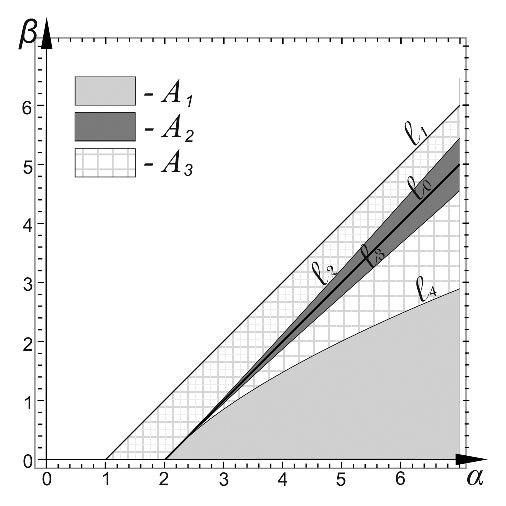
\includegraphics[width=0.55\linewidth]{neumanareas.eps} \\ Fig. 1: Regions with the same bifurcations }
\end{minipage}
\vspace{0.1cm}

The borders of regions depend on maximal amount of stable points, which are detected there for map \eqref{phi_map}. For values of parameters $ \alpha $ and $ \beta $ from region $ A_1 $ it is possible to exist five stable points (fig.2a). In regions $ A_2 $ and $ A_3 $ it is possible to exist seven (fig.2b) and six stable points (fig.2c), respectively.

\smallskip

\hspace{-1.5cm}
\begin{minipage}[h]{0.45\linewidth}
	\center{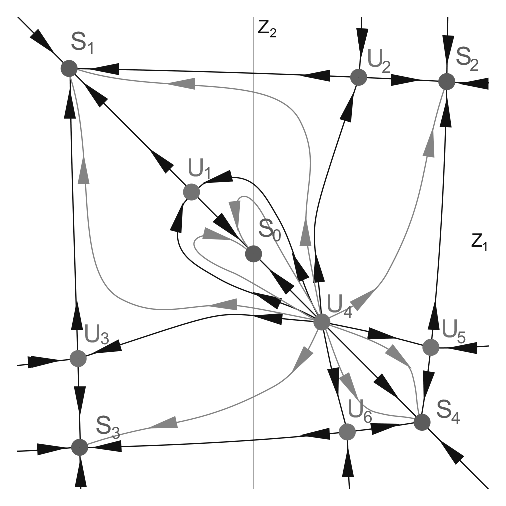
\includegraphics[width=0.6\linewidth]{neuman5.eps} \\ a) $ (\alpha, \beta) \in A_1 $ }
\end{minipage}
\hspace{-1.5cm}
\begin{minipage}[h]{0.45\linewidth}
	\center{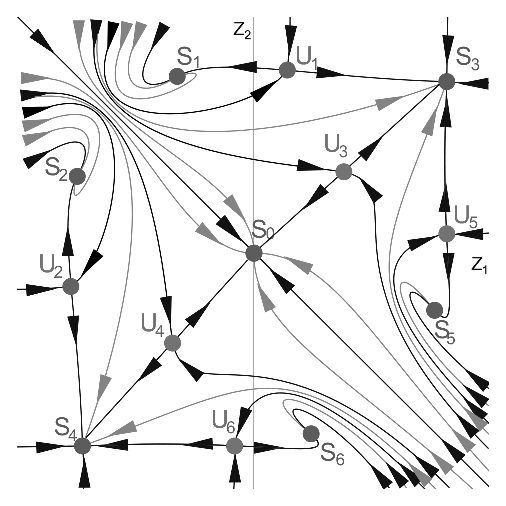
\includegraphics[width=0.6\linewidth]{neuman7.eps} \\ b) $ (\alpha, \beta) \in A_2 $ }
\end{minipage}
\hspace{-1.5cm}
\begin{minipage}[h]{0.45\linewidth}
	\center{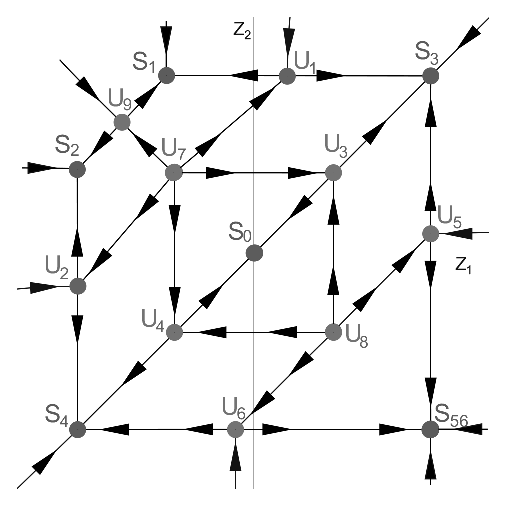
\includegraphics[width=0.6\linewidth]{neuman6.eps} \\ c) $ (\alpha, \beta) \in A_3 $ }
\end{minipage}
\begin{center}
	Fig. 2: Phase portraits of map
\end{center}	

The most important element for building of regions is line $ l_0 = \{ (\alpha, \beta): \beta = \alpha-2 \} $. Curves $ l_2 $ and $ l_3 $ are symmetric relative to line $ l_0 $ and touch each other in point $ (2, 0) $. These curves are borders of region $ A_2 = \{ (\alpha, \beta): \beta < l_2, \beta > l_3 \} $. Also in point $ (2, 0) $ curve $ l_4 $ traces to line $ l_0 $. It permits to determine region $ A_1 = \{ (\alpha, \beta): \beta < l_4, \beta > l_0 \} $. Doubly connected region $ A_3 = \{ (\alpha, \beta): \beta > l_2, \beta < l_1, \beta > l_4, \beta < l_3 \} $, where line $ l_1 = \{ (\alpha, \beta): \beta = \alpha-1 \} $ describes one of conditions for $ \alpha $ and $ \beta $ in system \eqref{u_system}.

In article [6] there are examples of different bifurcations for certain values of initial parameters.

In the case $ a_1 = 1, a_2 = 2, u_0 = u_3, u_1 = u_4 $ on coordinate plane of parameters $ (\alpha, \beta) $ there are regions $ A_1, A_2, A_3 $ and curves $ l_0, ..., l_3 $. They are shown on fig.3.

\hspace{1.5cm}
\begin{minipage}[h]{0.65\linewidth}
	\center{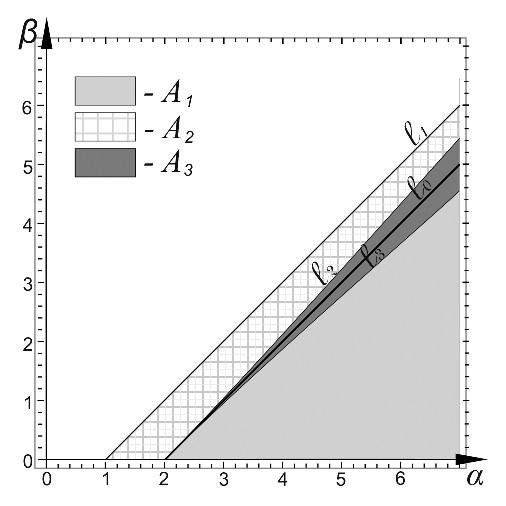
\includegraphics[width=0.55\linewidth]{periodicareas.eps} \\ Fig. 3: Regions with the same bifurcations }
\end{minipage}
\vspace{0.1cm}

In article [7] there are examples of different bifurcations for certain values of initial parameters.

For values of parameters $ \alpha $ and $ \beta $ from regions $ A_1 = \{ (\alpha, \beta): \beta > 0, \beta < l_3 \} $ (fig.4a) and $ A_2 = \{ (\alpha, \beta): \beta > l_2, \beta < l_1 \} $ (fig.4b) it is possible to exist seven stable points for map \eqref{phi_map}. The difference between these cases is the types of unstable points $ U_1, ..., U_6 $. In region $ A_3 = \{ (\alpha, \beta): \beta > l_3, \beta < l_2 \} $ there is an unstable manifold around zero balance state $ S_0 $ instead of unstable points $ U_1, ..., U_6 $. Every point of this manifold is an unstable state.

\hspace{0.5cm}
\begin{minipage}[h]{0.45\linewidth}
	\center{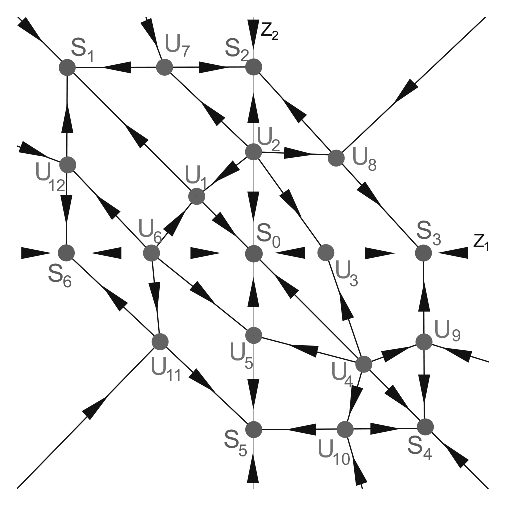
\includegraphics[width=0.6\linewidth]{periodic1.eps} \\ a) $ (\alpha, \beta) \in A_1 $ }
\end{minipage}
\hspace{-1cm}
\begin{minipage}[h]{0.45\linewidth}
	\center{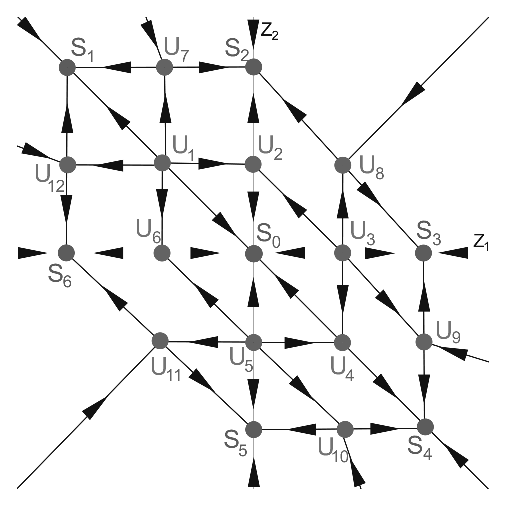
\includegraphics[width=0.6\linewidth]{periodic2.eps} \\ b) $ (\alpha, \beta) \in A_2 $ }
\end{minipage}
\begin{center}
	Fig. 4: Phase portraits of map
\end{center}

In the case $ a_1 = 0, a_2 = 1, u_1 = u_4 $ on coordinate plane of parameters $ (\alpha, \beta) $ there are regions $ A_1, A_2, A_3 $ and curves $ l_0, ..., l_5 $. They are shown on fig.5.

Line $ l_5 $ comes nearer to curve $ l_2 $, when parameter $ \alpha $ increases. Curves $ l_0, ..., l_5 $ permit to describe regions $ A_1 = \{ (\alpha, \beta): \beta>0, \beta<l_4, \beta>l_2, \beta<l_5 \} , A_2 = \{ (\alpha, \beta): \beta>0, \beta<l_4, \beta>l_2, \beta<l_5 \} $ and $ A_3 = \{ (\alpha, \beta): \beta > l_3, \beta < l_2  \} $.

\hspace{1.5cm}
\begin{minipage}[h]{0.65\linewidth}
	\center{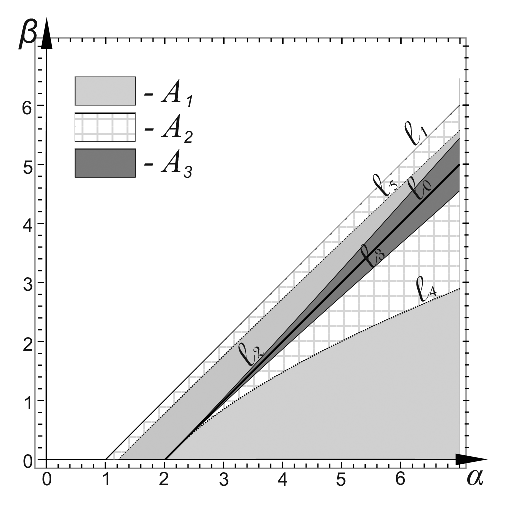
\includegraphics[width=0.55\linewidth]{uniwaveareas.eps} \\ Fig. 5: Regions with the same bifurcations }
\end{minipage}
\vspace{0.1cm}

For every region $ A_1, A_2 $ and $ A_3 $, as in articles [6, 7] there were given all possible bifurcations in a phase space of map \eqref{phi_map}. The difference is the bifurcational value of $ d $. Let us consider one sequence of bifurcations for parameters $ (\alpha, \beta) \in A_2 $ in details.

For any fixed values $ (\alpha, \beta) \in A_2 $ and change of parameter $ d $ in a phase space of map \eqref{phi_map} there is the only sequence of bifurcations. Let us fix values $ \alpha = 1.9 $ and $ \beta = 0.1 $, parameter $ d $ will increase. As a result, there is the following sequence of bifurcations:

\hspace{-1.0cm}
\begin{minipage}[h]{0.65\linewidth}
	\center{\includegraphics[width=0.55\linewidth]{uniwave1.eps} \\ a) $ d < d_1 $ }
\end{minipage}
\hspace{-3.0cm}
\begin{minipage}[h]{0.65\linewidth}
	\center{\includegraphics[width=0.55\linewidth]{uniwave2.eps} \\ b) $ d_1 < d < d_2 $ }
\end{minipage}
\begin{center}
	Fig. 6: Phase portraits of map
\end{center}

\begin{enumerate}

\item $ d < d_1, d_1\approx0.316 $: map \eqref{phi_map} has 4 stable and 9 unstable points (fig.6a)
\item $ d = d_1 $: unstable saddles $ U_7, U_8 $ and $ U_9 $ come nearer to stable saddles $ S_1, S_2 $ and $ S_3 $, merge with them and stable manifold $ M_S $ appears. The movement on manifold $ M_S $ is clockwise. Unstable points $ U_1, U_3 $ and $ U_5 $ become focuses.
\item $ d_1 < d < d_2, d_2\approx0.317 $: map \eqref{phi_map} has 1 stable, 3 unstable points and stable manifold (fig.6b).
\item $ d = d_2 $: unstable manifolds separate from unstable focuses $ U_1, U_3, U_5 $. Points $ U_1, U_3 $ and $ U_5 $ become stable focuses $ S'_1, S'_2 $ and $ S'_3 $.
\item $ d_2 < d < d_3, d_3\approx0.3174 $: map \eqref{phi_map} has 4 stable and 3 unstable points. Also it has 1 stable and 3 unstable manifolds (fig.7a).
\item $ d = d_3 $: 3 unstable manifolds around stable focuses $ S'_1, S'_2 $ and $ S'_3 $ merge with stable manifold $ M_S $. All manifolds disappear.
\item $ d_3 < d < d_4, d_4\approx0.3178 $: map \eqref{phi_map} has 4 stable and 3 unstable points (fig.7b).

\hspace{-1.0cm}
\begin{minipage}[h]{0.65\linewidth}
	\center{\includegraphics[width=0.55\linewidth]{uniwave3.eps} \\ a) $ d_2 < d < d_3 $ }
\end{minipage}
\hspace{-3.0cm}
\begin{minipage}[h]{0.65\linewidth}
	\center{\includegraphics[width=0.55\linewidth]{uniwave4.eps} \\ b) $ d_3 < d < d_4 $ }
\end{minipage}
\begin{center}
	Fig. 7: Phase portraits of map
\end{center}
\item Last bifurcation takes places, when $ d = d_4 $. Unstable saddles $ U_2, U_4 $ and $ U_6 $ merge with stable focuses $ S'_2, S'_3 $ and $ S'_1 $ and disappear. When $ d > d_4 $ map \eqref{phi_map} has only zero balance state $ S_0 $.

\end{enumerate}

\begin{thebibliography}{20}

\bibitem{GlKolRoz2011} S.~D.~Glyzin, A.~Yu.~Kolesov, N.~Kh.~Rozov,  
\textit{Relaxation self-oscillations in neuron systems. II},
Differential Equations \textbf{47} (12), 1697--1713 (2011). 

\bibitem{GlKolRoz2012} S.~D.~Glyzin, A.~Yu.~Kolesov, N.~Kh.~Rozov,  
\textit{Relaxation self-oscillations in neuron systems. III},
Differential Equations \textbf{48} (2), 159--175 (2012).

\bibitem{GlKolRoz2015UMN} S.~D.~Glyzin, A.~Yu.~Kolesov, N.~Kh.~Rozov, 
\textit{Self-excited relaxation oscillations in networks of impulse neurons}, 
Russian Math. Surveys \textbf{70} (3), 383--452 (2015).

\bibitem{GlKolRoz2015MAIS} S.~D.~Glyzin, A.~Yu.~Kolesov, N.~Kh.~Rozov,  
\textit{Self-excited wave processes in chains of unidirectionally coupled impulse neurons},
Model. Anal. Info. Sist. \textbf{22} (3), 404--419 (2015).

\bibitem{GlKolRoz2016} 
S.~D.~Glyzin, A.~Yu.~Kolesov, N.~Kh.~Rozov, 
\textit{Self-Sustained Relaxation Oscillations in Time-Delay Neural Systems}, 
Journal of Physics: Conference Series. \textbf{727} (012004) (2016).

\bibitem{IS} L.~I.~Ivanovsky, S.~O.~Samsonov,  
\textit{Dynamics of two-dimensional mapping and stable regimes of singularly perturbed neuron system},
Computer technologies in sciences. Methods of simulations on supercomputers. Part 2. Proceedings, 121--132 (2015) [in Russian].

\bibitem{I} L.~I.~Ivanovsky, 
\textit{Dynamic properties of one class of impulse systems},
Computer technologies in sciences. Methods of simulations on supercomputers. Part 3. Proceedings, 126 -- 131 (2015) [in Russian].

\end{thebibliography}

\end{document}
